\documentclass[journal,12pt,onecolumn]{IEEEtran}
\usepackage{cite}
\usepackage{graphicx}
\usepackage{amsmath,amssymb,amsfonts,amsthm}
\usepackage{algorithmic}
\usepackage{graphicx}
\usepackage{textcomp}
\usepackage{xcolor}
\usepackage{txfonts}
\usepackage{listings}
\usepackage{enumitem}
\usepackage{mathtools}
\usepackage{gensymb}
\usepackage{comment}
\usepackage[breaklinks=true]{hyperref}
\usepackage{tkz-euclide} 
\usepackage{listings}
\usepackage{gvv}                                        
%\def\inputGnumericTable{}                                 
\usepackage[latin1]{inputenc} 
\usetikzlibrary{arrows.meta, positioning}
\usepackage{xparse}
\usepackage{color}                                            
\usepackage{array}                                            
\usepackage{longtable}                                       
\usepackage{calc}                                             
\usepackage{multirow}
\usepackage{multicol}
\usepackage{hhline}                                           
\usepackage{ifthen}                                           
\usepackage{lscape}
\usepackage{tabularx}
\usepackage{array}
\usepackage{float}
\newtheorem{theorem}{Theorem}[section]
\newtheorem{problem}{Problem}
\newtheorem{proposition}{Proposition}[section]
\newtheorem{lemma}{Lemma}[section]
\newtheorem{corollary}[theorem]{Corollary}
\newtheorem{example}{Example}[section]
\newtheorem{definition}[problem]{Definition}
\newcommand{\BEQA}{\begin{eqnarray}}
\newcommand{\EEQA}{\end{eqnarray}}
\usepackage{float}
\usepackage{caption}

%\newcommand{\define}{\stackrel{\triangle}{=}}
\theoremstyle{remark}
\usepackage{circuitikz}
\usepackage{tikz}
\graphicspath{{figs/}}
\usepackage[top=1in,bottom=1in,left=1in,right=1in]{geometry}
\pagestyle{empty}
\setlength{\parindent}{0pt}

\title{PI: PRODUCTION AND INDUSTRIAL ENGINEERING}
\author{EE25BTECH11023-Venkata Sai}
\begin{document}
\maketitle
 
\textbf{Q. 1 - Q. 20 carry one mark each.}

\begin{enumerate}

\item The homogeneous part of the differential equation
$\frac{d^2 y}{dx^2} + p \frac{dy}{dx} + q y = r$
has real distinct roots if $\brak{p, q and r are constants}$
\begin{enumerate}
\begin{multicols}{2}
\item $p^2 - 4q > 0$  
\item  $p^2 - 4q < 0$ 
\item  $p^2 - 4q = 0$ 
\item  $p^2 - 4q = r$ 
\end{multicols}
\end{enumerate}
\hfill (GATE PI 2009) 
\item The total derivative of the function $xy$ is
\begin{enumerate}
\begin{multicols}{2}
\item $x dy + ydx$ 
\item $xdx + ydy$ 
\item  $dx + dy$ 
\item $dx dy$ 
\end{multicols}
\end{enumerate}
\hfill (GATE PI 2009) 
\item A helical compression spring has: $ d = $wire diameter, $ D = $ mean coil diameter, $ E = $ Young's modulus, $ G = $ modulus of rigidity and $ N_a = $ number of active coils. The spring stiffness is
\begin{enumerate}
\begin{multicols}{2}
\item $\frac{d E}{8 D^{3} N_a}$  
\item $\frac{d G}{8 D^{3} N_a}$ 
\item  $\frac{d^{3} E}{8 D N_a}$ 
\item $\frac{d^{3}}{8 D N_a}$ 

\end{multicols}
\end{enumerate}
\hfill (GATE PI 2009)
\item Which of the following processes is NOT executed by an ideal Rankine cycle with no superheat?
\begin{enumerate}
\item Isentropic expansion
\item Isentropic compression
\item Constant temperature heat addition
\item Constant temperature heat rejection
\end{enumerate}
\hfill (GATE PI 2009)
\item During the numerical solution of a first order differential equation using the Euler (also known as Euler Cauchy) method with step size $h$, the local truncation error is of the order of
\begin{enumerate}
\begin{multicols}{4}
\item  $h^2$ 
\item $h^3$ 
\item $h^4$ 
\item $h^5$ 
\end{multicols}
\end{enumerate}
\hfill (GATE PI 2009)
\item For a granted patent to last for 20 years, the patent must be
\begin{enumerate}
\begin{multicols}{2}
\item owned by the inventor 
\item renewed and maintained \\
\item novel 
\item  non-obvious \\
\end{multicols}
\end{enumerate}

\hfill (GATE PI 2009)
\item As per Kendall's notation in M/G/c queuing system, the number of arrivals in a fixed time follows
\begin{enumerate}
\begin{multicols}{2}
\item  Beta distribution 
\item  Normal distribution 
\item Poisson distribution 
\item Uniform distribution 
\end{multicols}
\end{enumerate}
\hfill (GATE PI 2009)
\item Which of the following forecasting models explicitly accounts for seasonality of demand?
\begin{enumerate}
\begin{multicols}{2}
\item Simple moving average  model 
\item Simple exponential smoothing model \\
\item Holt's model 
\item Winter's model \\
\end{multicols}
\end{enumerate}
\hfill (GATE PI 2009)
\item A typical Fe-C alloy containing greater than 0.8\% C is known as
\begin{enumerate}
\begin{multicols}{2}
\item Eutectoid steel 
\item Hypoeutectoid steel 
\item Mild steel 
\item Hypereutectoid steel 
\end{multicols}
\end{enumerate}
\hfill (GATE PI 2009)
\item The capacity of a material to absorb energy when deformed elastically, and to release it back when unloaded is termed as
\begin{enumerate}
\begin{multicols}{2}
\item toughness 
\item resilience 
\item  ductility 
\item malleability 
\end{multicols}
\end{enumerate}
\hfill (GATE PI 2009)
\item The product of the complex numbers $\brak{3 - i2}$ and $\brak{3 + i4}$ results in
\begin{enumerate}
\begin{multicols}{4}
\item $\brak{1 + i^6}$ 
\item $\brak{9-i^8}$  
\item $\brak{9+i^8}$ 
\item $\brak{17 + i^6}$ \\
\end{multicols}
\end{enumerate}
\hfill (GATE PI 2009)
\item The value of the determinant
$
\myvec{
4 & 1 & 1 \\
2 & 1 & 3 \\
1 & 3 & 2
}
$
is
\begin{enumerate}
\begin{multicols}{4}
\item -28 
\item -24 
\item 32 
\item 36 
\end{multicols}
\end{enumerate}

\hfill (GATE PI 2009)

\item If module and number of teeth of a spur gear with involute profile are 3 mm and 23 respectively, then the pitch diameter (in mm) of the spur gear is
\begin{enumerate}
\begin{multicols}{4}
\item  7.67 
\item 15.34 
\item 34.50 
\item 69.00 
\end{multicols}
\end{enumerate}
\hfill (GATE PI 2009)
\item Hot chamber die casting process is NOT suited for
\begin{enumerate}
\begin{multicols}{2}
\item Lead and its alloys 
\item Zinc and its alloys 
\item Tin and its alloys  
\item Aluminum and its alloys 
\end{multicols}
\end{enumerate}
\hfill (GATE PI 2009)
\item The total angular movement (in degrees) of a lead-screw with a pitch of 5.0 mm to drive the work-table by a distance of 200 mm in a NC machine is \\
\begin{enumerate}
\begin{multicols}{4}
\item  14400 
\item  28800
\item 57600 
\item 72000 
 \end{multicols}
 \end{enumerate}
\hfill (GATE PI 2009)
\item Anisotropy in rolled components is caused by
\begin{enumerate}
\begin{multicols}{2}
\item change in dimensions 
\item scale formation 
\item closure of defects 
\item grain orientation 
\end{multicols}
\end{enumerate}
\hfill (GATE PI 2009)
\item Which of the following processes is used to manufacture products with controlled porosity?
\begin{enumerate}
\begin{multicols}{2}
\item Casting 
\item Welding 
\item Forming 
\item Powder metallurgy 
\end{multicols}
\end{enumerate}
\hfill (GATE PI 2009)
\item Which of the following powders should be fed for effective oxy-fuel cutting of stainless steel?
\begin{enumerate}
\begin{multicols}{4}
\item  Steel
\item Aluminum
\item Copper 
\item Ceramic 
\end{multicols}
\end{enumerate}
\hfill (GATE PI 2009)
\item An autocollimator is used to

\begin{enumerate}
\item measure small angular displacements on flat surfaces
\item compare known and unknown dimensions
\item measure the flatness error
\item measure roundness error between centers
\end{enumerate}
\hfill (GATE PI 2009)
\item Diamond cutting tools are not recommended for machining of ferrous metals due to

\begin{enumerate}
\item high tool hardness
\item high thermal conductivity of work material
\item poor tool toughness
\item chemical affinity of tool material with iron
\end{enumerate}
\hfill (GATE PI 2009)
\item The value of $x_3$ obtained by solving the following system of linear equations is
\begin{align*} 
x + 2x_2 - 2x_3 = 4 \\ 
2x + x_2 + x_3 = -2 \\
-x + x_2 - x_3 = 2
\end{align*}
\begin{enumerate}
\begin{multicols}{2}
\item -12 
\item -2 
\item 0 
\item 12 
\end{multicols} 
\end{enumerate}
\hfill (GATE PI 2009)
\item The displacement and acceleration of a cam follower mechanism are plotted in the following figures:

\begin{figure}[h]
    \centering
    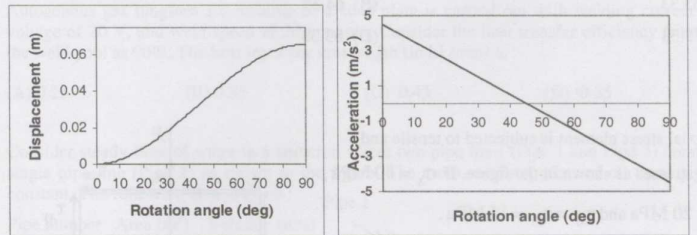
\includegraphics[width=0.5\linewidth]{figs/1.png}
    \caption{}
    \label{fig:placeholder}
\end{figure} 

The nature of the displacement curve is:
\begin{enumerate}
\begin{multicols}{2}
\item Cubic 
\item Quadratic 
\item Simple harmonic 
\item Linear 
\end{multicols}
\end{enumerate}
\hfill (GATE PI 2009)
\item The solution of the differential equation
$
\frac{d^2 r}{dx^2} = 0
$
with boundary conditions: (i) $\frac{dy}{dx} = 1$ at $x = 0$, (ii) $\frac{dy}{dx} = 1$ at x=1 is
\begin{enumerate}
\item $y = 1$ 
\item $y = x$ 
\item $y = x + C$, where $C$ is an arbitrary constant  
\item $y = C_1 x + C_2$, where $C_1, C_2$ are arbitrary constants 

\end{enumerate}
\hfill (GATE PI 2009)
\item The line integral of the vector function $\mathbf{F} = 2x + x^2 \mathbf{\hat{j}}$ along the x-axis from $x=1$ to $x=2$ is
\begin{enumerate}
\begin{multicols}{4}
\item 0
\item 2.33
\item 3
\item 5.33 
\end{multicols}
\end{enumerate}

\hfill (GATE PI 2009)
\item Using direct extrusion process, a round billet of 100 mm length and 50 mm diameter is extruded. Considering an ideal deformation process (no friction and no redundant work), extrusion ratio 4, and average flow stress of material 300 MPa, the pressure (in MPa) on the ram will be
\begin{enumerate}
\begin{multicols}{4}
\item 416
\item 624
\item 700
\item 832
\end{multicols}
\end{enumerate}
\hfill (GATE PI 2009)
\item A friction clutch is designed to transmit 15 horsepower at 1500 rpm. The torque (in N·m) experienced by the clutch is
\begin{enumerate}
\begin{multicols}{2}
\item 1.19 
\item 7.46 
\item 71.24 
\item 447.61 
\end{multicols}
\end{enumerate}
\hfill (GATE PI 2009)
\item A manufacturer has set up an assembly line where first, Task I is performed in Workstation 1 for 0.3 minutes; then Task II is performed in Workstation 2 for 0.4 minutes; and finally Task III is performed in Workstation 3 for 0.3 minutes. The efficiency (in \%) of this assembly line setup is
\begin{enumerate}
\begin{multicols}{2}
\item  33.33 
\item 64.33 
\item 75.33
\item 83.33 
\end{multicols}
\end{enumerate}
\hfill (GATE PI 2009)

\item A biaxial stress element is subjected to tensile and shear stresses as shown in the figure. If $\sigma_1 = 40$ MPa, $\sigma_y = 20$ MPa and $T_{xy} = T_{yx} = 15$ MPa. The principal normal stresses (in MPa) are:

\begin{figure}[h]
    \centering
    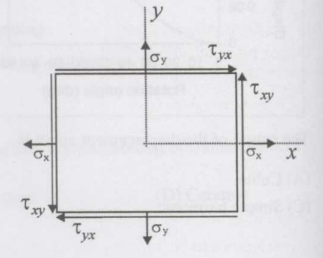
\includegraphics[width=0.5\linewidth]{figs/2.png}
    \caption{}
    \label{fig:placeholder}
\end{figure} 

\begin{enumerate}
\begin{multicols}{2}
\item 5 and 55
\item 10 and 30 
\item 12 and 48
\item 20 and 40
\end{multicols}
\end{enumerate}
\hfill (GATE PI 2009)

\item The area under the curve shown, between $x=1$ and $x=3$, to be evaluated using the trapezoidal rule. The following points on the curve are given:

\begin{center}
\begin{table}[htbp]
  \centering
  \caption{Table-3}
  \label{table3}
  \begin{tabular}{cc}
  \textbf{Processing Technique} & \textbf{Producct} \\ \\
    P. Calendering & 1. Pipes \\
    Q. Extrusion & 2. Disposable cups \\
    R. Injection moulding & 3. Sheets \\
    S. Thermoforming & 4. Nylon gears \\
  \end{tabular}
\end{table}
\end{center}

\begin{figure}[h]
    \centering
    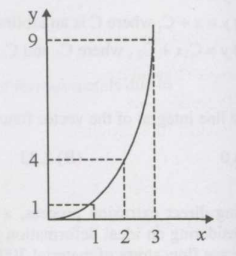
\includegraphics[width=0.3\linewidth]{figs/3.png}
    \caption{}
    \label{fig:placeholder}
\end{figure} 
\begin{center}

\end{center}
The evaluated area (in m$^2$) will be
\begin{enumerate}
\begin{multicols}{4}
\item 7  
\item 8.67 
\item 9  
\item 18 
\end{multicols}
\end{enumerate}
\hfill (GATE PI 2009)
\item The pressure drop for laminar flow of a liquid in a smooth pipe at normal temperature and pressure is
\begin{enumerate}
\begin{multicols}{2}
\item directly proportional to density 
\item inversely proportional to density 
\item independent of density 
\item proportional to density$^{0.75}$

\end{multicols}
\end{enumerate}
\hfill (GATE PI 2009)
\item A titanium sheet of 5.0 mm thickness is cut by wire-cut EDM process using a wire of 1.0 mm diameter. A uniform spark gap of 0.5 mm on both sides of the wire is maintained during cutting operation. If the feed rate of the wire into the sheet is 20 mm/min, the material removal rate (in mm$^3$/min) will be
\begin{enumerate}
\begin{multicols}{4}
\item 150 
\item 200
\item 300 
\item 400 
\end{multicols}
\end{enumerate}
\hfill (GATE PI 2009)
\item Autogenous gas tungsten arc welding of a steel plate is carried out with welding current of 500 A, voltage of 20 V, and weld speed of 20 mm/min. Consider the heat transfer efficiency from the arc to the weld pool as 90\%. The heat input per unit length (in kJ/mm) is
\begin{enumerate}
\begin{multicols}{4}
\item  0.25 
\item 0.35 
\item 0.45 
\item 0.55 
\end{multicols}
\end{enumerate}

\hfill (GATE PI 2009)
\item Consider steady flow of water in a situation where two pipe lines (Pipe 1 and Pipe 2) combine into a single pipeline (Pipe 3) as shown in the figure. The cross-sectional areas of all three pipelines are constant. The following data is given : \\
\begin{center}
\begin{tabular}{|c|c|c|}
     \hline
     \textbf{Mineral} & \textbf{Modal abundance \brak{\%}} & \textbf{Partition coefficient}\\
     \hline
     Clinopyroxene & $45$ & $0.506$ \\
      \hline
      Orthopyroxene & $40$ & $0.42$ \\
      \hline
      Olivine & $10$ & $0.045$ \\
      \hline
      Plagioclase & $05$ & $0.019$ \\
      \hline
\end{tabular}
\end{center}
Assuming water properties and velocities to be uniform across the cross sections of the inlets and the outlet, the exit velocity (in m/s) in pipe 3 is
\begin{enumerate}
\begin{multicols}{4}
\item  1 
\item 1.5 
\item  2  
\item 2.5
\end{multicols}
\end{enumerate}
\hfill (GATE PI 2009)

\item Match the Following:
{
\setlength{\columnsep}{-5cm}
\begin{multicols}{2}
\begin{enumerate}[label=\Alph*.]
    \item[]  \textit{\textbf{Group I (Product)}}
    \item Process layout
    \item Product flow layout
    \item Fixed position layout
    \item Cellular layout 
\end{enumerate}
\columnbreak
\begin{enumerate}[label=\arabic*.]
    \item[] \textit{\textbf{Group II (Manufacturing Process)}}
    \item Inflexible to significant changes in product design
    \item Distinct part families and expanded worker training
    \item Low equipment utilization and high skill requirement
    \item Large work-in-process and increased material handling
\end{enumerate}
\end{multicols}
}
\begin{multicols}{2}
\begin{enumerate}
    \item P-4, Q-1, R-3, S-2
    \item P-4, Q-3, R-2, S-1
    \item P-2, Q-1, R-4, S-3
    \item P-1, Q-4, R-3, S-2
\end{enumerate}
\end{multicols}
\hfill (GATE PI 2009)
\item Consider the joint probability mass function of random variables X and Y as shown in the table below: \\
For instance, $P\cbrak{X=1, Y=2}$ = 0.3
\begin{center}
\begin{center}
\begin{tabular}{ll}
    \textbf{Group I} & \textbf{Group II} \\
    P. Ferrite & 1. Hexagonal Close Packed (HCP) \\
    Q. Austenite & 2. Body Centered Cubic (BCC) \\
    R. Martensite & 3. Body Centered Tetragonal (BCT) \\
    & 4. Face Centered Cubic (FCC)
\end{tabular}
\end{center}
\end{center}
The value of $P\cbrak{X=2|Y=2}$ is

\begin{enumerate}
\begin{multicols}{4}
\item 0.10 
\item 0.25 
\item 0.40 
\item 0.75 
\end{multicols}
\end{enumerate}

\hfill (GATE PI 2009)
\item A grocery store faces a demand of 50 units of soap per day. The store orders soap periodically. It costs Rs. 100 to initiate a purchase order. It costs Rs. 0.04 per soap per day to store the soap. The lead time between placing and receiving the order is 4 days. The optimal inventory policy for ordering soap is to
\begin{enumerate}
\item order 500 units when inventory drops to 200 units 
\item order 500 units when inventory drops to 100 units
\item order 1000 units when inventory drops to 200 units
\item order 1000 units when inventory drops to 100 units
\end{enumerate}
\hfill (GATE PI 2009)
\item A disk of 200 mm diameter is blanked from a strip of an aluminum alloy of thickness 3.2 mm. The material shear strength to fracture is 150 MPa. The blanking force (in kN) is

\begin{enumerate}
\begin{multicols}{4}
\item 291 
\item 301 
\item 311 
\item 321 
\end{multicols}
\end{enumerate}

\hfill (GATE PI 2009)

\item Match the following:

\noindent
\begin{multicols}{2}
\begin{enumerate}[label=\Alph*.]
    \item[]  \textit{\textbf{Group I (Product)}}
    \item Refrigerator liners
    \item Composite pressure vessels
    \item Hollow parts of thermoset plastics
    \item Rubber sheets
\end{enumerate}
\columnbreak
\begin{enumerate}[label=\arabic*.]
    \item[] \textit{\textbf{Group II (Manufacturing Process)}}
    \item Filament winding
    \item Thermoforming
    \item Calendering
    \item Rotational moulding
\end{enumerate}
\end{multicols}


\begin{multicols}{2}
\begin{enumerate}
    \item P-2, Q-1, R-4, S-3
    \item P-1, Q-2, R-3, S-4
    \item P-1, Q-4, R-2, S-3
    \item P-2, Q-4, R-1, S-3
\end{enumerate}
\end{multicols}
\hfill (GATE PI 2009)
\noindent 
\item Match the following:
{
\setlength{\columnsep}{-8cm}
\begin{multicols}{2}
\begin{enumerate}[label=\Alph*.]
    \item[]  \textit{\textbf{Group I (Device)}}
    \item Jig
    \item Fixture
    \item Clamp
    \item Locator
\end{enumerate}
\columnbreak
\begin{enumerate}[label=\arabic*.]
    \item[] \textit{\textbf{Group II (Function)}}
    \item Helps to place the workpiece in the same position cycle after cycle
    \item Holds the workpiece only
    \item Holds and positions the workpiece
    \item Holds and positions the workpiece and guides the cutting tool during a machining operation
\end{enumerate}
\end{multicols}
}

\begin{multicols}{2}
\begin{enumerate}
    \item P-4, Q-3, R-1, S-2
    \item P-1, Q-2, R-3, S-4
    \item P-1, Q-4, R-3, S-2
    \item P-4, Q-3, R-2, S-1
\end{enumerate}
\end{multicols}
\hfill (GATE PI 2009)
\item A spur gear having a pressure angle of $20\degree$, module of 4 mm and 40 teeth is to be inspected for its pitch circle diameter using two rollers (test plug method). If the centres of the rollers lie on the pitch circle, the suitable roller diameter (in mm) and the resulting distance (in mm) between the rollers placed in opposite spaces will respectively be
\begin{enumerate}
\begin{multicols}{2}
\item 2.9 and 82.9 
\item 2.9 and 165.9 
\item 5.9 and 82.9 
\item 5.9 and 165.9 
\end{multicols}
\end{enumerate}
\hfill (GATE PI 2009)
\item A company makes a product using three independent components I, II and III, with reliabilities of 0.80, 0.85 and 0.90 respectively. If the company decides to add one redundant unit of component I to improve reliability, then the reliability of the product is
\begin{enumerate}
\begin{multicols}{4}
\item  0.612 
\item 0.734 
\item 0.837 
\item 0.969
\end{multicols}
\end{enumerate}

\hfill (GATE PI 2009)
\item Given: \\
Assertion [a] : Managers spend time on job analysis and job rating.\\
Reason [r]: Scientific management of wage structures through job evaluation helps increase productivity.
\begin{enumerate}
\item Both [a] and [r] are true and [r] is the correct reason for [a].
\item Both [a] and [r] are true, but [r] is not the correct reason for [a].
\item Both [a] and [r] are false. 
\item \text[a] is true but [r] is false.
\end{enumerate}
\hfill (GATE PI 2009)
\item A spare parts retail shop has sales of Rs. 4,00,000 and a profit of Rs. 50,000 for a product, in its first quarter. The profit volume (PV) ratio is 25\%. The margin of safety = profit / PV ratio. The break even point of sales (in Rs.) is
\begin{enumerate}
\begin{multicols}{2}
\item 20,000 
\item 40,000 
\item 2,00,000 
\item 4,00,000 
\end{multicols}
\end{enumerate}
\hfill (GATE PI 2009)
\item The following information relates to worker's payment in a company: \\
\centerline{Standard production of a worker = 12 jobs per hour} \\
\centerline{Standard job rate = Rs. 3.00 per job}\\
\centerline{Pay for production less than standard = 85\% of standard job rate}\\
\centerline{Pay for production more than standard = 120\% of standard job rate} \\
Three workers produce at the rate of 11, 13 and 15 jobs per hour. The total pay for three workers per hour based on differential wage incentive scheme is
\begin{enumerate}
\begin{multicols}{2}
\item  Rs. 117.00 
\item Rs. 128.85 
\item  Rs. 1404.00 
\item  Rs. 1546.20 
\end{multicols}
\end{enumerate}
\hfill (GATE PI 2009)
\item{Match the following:}

\noindent
\begin{multicols}{2}
\begin{enumerate}[label=\Alph*.]
    \item[]  \textit{\textbf{Group I (Protection type)}}
    \item Patent
    \item Trademark
    \item Copyright
    \item Industrial design
\end{enumerate}
\columnbreak
\begin{enumerate}[label=\arabic*.]
    \item[] \textit{\textbf{Group II (Example in the Indian context)}}
    \item Manual of a product
    \item Appearance of an MP3 player
    \item Logo of a company
    \item Microprocessor
\end{enumerate}
\end{multicols}

\begin{multicols}{2}
\begin{enumerate}
    \item P-2, Q-4, R-3, S-1
    \item P-4, Q-1, R-3, S-2
    \item P-2, Q-3, R-4, S-1
    \item P-4, Q-3, R-1, S-2
\end{enumerate}
\end{multicols}
\hfill (GATE PI 2009)
\item{Match the following:}
{
\setlength{\columnsep}{-2cm}
\begin{multicols}{2}
\begin{enumerate}[label=\Alph*.]
    \item[]  \textit{\textbf{Group I (Design aspect)}}
    \item Form design
    \item Concurrent engineering
    \item Value analysis
    \item Product life cycle
\end{enumerate}
\columnbreak
\begin{enumerate}[label=\arabic*.]
    \item[] \textit{\textbf{Group II (Description)}}
    \item Introduction, growth, maturity and decline
    \item Determines cost of each function of the design
    \item Integration of product design and manufacturing
    \item Appearance, shape, colour and size of product
\end{enumerate}
\end{multicols}
}
\begin{multicols}{2}
\begin{enumerate}
    \item P-4, Q-1, R-2, S-3
    \item P-3, Q-2, R-4, S-1
    \item P-4, Q-3, R-2, S-1
    \item P-4, Q-2, R-3, S-1
\end{enumerate}
\end{multicols}
\hfill (GATE PI 2009)
\item In an orthogonal machining operation, the tool life obtained is 10 min at a cutting speed of 100 m/min, while at 75 m/min cutting speed, the tool life is 30 min. The value of index $n$ in the Taylor's tool life equation is
\begin{enumerate}
\begin{multicols}{2}
\item 0.262 
\item 0.323 
\item  0.423 
\item 0.521 
\end{multicols}
\end{enumerate}
\hfill (GATE PI 2009)
\item A solid cylinder of diameter D and height equal to D, and a solid cube of side L are being sand cast by using the same material. Assuming there is no superheat in both cases, the ratio of solidification time of the cylinder to that of the cube is
\begin{enumerate}
\begin{multicols}{2}
\item $\brak{L/D}^2$
\item  $\brak{2L/D}^2$ 
\item  $\brak{2D/L}^2$ 
\item $\brak{D/L}^2$ 
\end{multicols}
\end{enumerate}
\hfill (GATE PI 2009)
\item Following are some possible characteristics of a pile of powder mixture: \\
P. Low inter-particle friction \\
Q. High inter-particle friction \\
R. Low porosity \\
S. High porosity \\
If the angle of repose for a pile of powder mixture is low, it will exhibit
\begin{enumerate}
\begin{multicols}{2}
\item P and R 
\item P and S 
\item  Q and S 
\item Q and R 
\end{multicols}
\end{enumerate}
\hfill (GATE PI 2009)
\item Match the following:

\begin{multicols}{2}
\begin{enumerate}[label=\Alph*.]
    \item[]  \textit{\textbf{Group I}}
    \item Relational DBMS
    \item Primary key
    \item Retrieving data
    \item Boolean search
\end{enumerate}
\columnbreak
\begin{enumerate}[label=\arabic*.]
    \item[] \textit{\textbf{Group II}}
    \item SQL
    \item AND, OR
    \item Tables, columns and rows
    \item Columns that uniquely identify a row
\end{enumerate}
\end{multicols}


\begin{multicols}{2}
\begin{enumerate}
    \item P-3, Q-4, R-2, S-1
    \item P-3, Q-1, R-4, S-2
    \item P-3, Q-4, R-1, S-2
    \item P-4, Q-1, R-2, S-3 
\end{enumerate}
\end{multicols}
\hfill (GATE PI 2009) \\

\textbf{\large{Common Data Questions}}

\textbf{Common Data for Questions 51 and 52:}

Consider the Linear Programming Problem (LPP)\\
Maximize  $ z = 4x_1 + 3x_2 + 2x_3 $ \\
Subject to:
\begin{align*}
2x_1 + x_2 + 2x_3 \leq 50\  \text{(constraint 1)}   \\ 
x_1 + x_2 + x_3 \leq 30\  \text{(constraint 2)} \\
x_1, x_2, x_3 \geq 0  
\end{align*}
The associated simplex tableau at optimality is shown below, where $s_1$ and $s_2$ represent the slacks for constraints 1 and 2 respectively.

\begin{center}
\begin{center}
\begin{tabular}{|c|c|c|}
    \hline
    Task & Task time (Seconds) & Immediate predecessor(s) \\
    \hline
    P & 20 & - \\ \hline
    Q & 25 & P \\  \hline
    R & 10 & Q \\ \hline
    S & 15 & Q \\ \hline 
    T & 25 & R, S \\    \hline
\end{tabular}
\end{center}
\end{center}

\item Basic variables in the optimal solution are
\begin{enumerate}
\begin{multicols}{2}
\item  $s_1\ \text{and}\ s_2$ 
\item $x_1\ \text{and}\ x_2$ 
\item  $x_1, x_2\ \text{and}\ x_3$ 
\item $x_3, s_1\ \text{and}\ s_2$ 
\end{multicols}
\end{enumerate}
\hfill (GATE PI 2009)
\item Suppose that in the LPP given, the right hand side of constraint 1 changes from 50 to 40. The new objective value is
\begin{enumerate}
\begin{multicols}{4}
\item 90 
\item  100 
\item 110 
\item 120 
\end{multicols}

\end{enumerate}
\hfill (GATE PI 2009) \\
\textbf{Common Data for Questions 53 and 54:}


In acceptance sampling, the probability distribution of the number of defectives X in a sample can be approximated as a Poisson distribution
\begin{align*} 
\text{Prob}\cbrak{X = k}  = \frac{(np)^k e^{-np}}{k!}\ k=0,1,2,...
\end{align*}
where $n$ is the sample size and $p$ is the actual proportion or percent of defective items in a batch.\\

A company receives a shipment batch of $N = 2000$ items. The sampling plan followed by the company is to sample $n = 50$ items from the batch and accept the batch if the number of defective items is 2 or less. Let the Acceptable Quality Level (AQL) be 0.02 and the Lot Tolerance Percent Defective (LTPD) be 0.05.


\item The probability of incorrectly rejecting a good batch or the Producer's risk is
\begin{enumerate}
\begin{multicols}{2}
\item 0.0805 
\item 0.3678 
\item 0.5437 
\item 0.9195 
\end{multicols}
\end{enumerate}
\hfill (GATE PI 2009)
\item The probability of incorrectly accepting a bad batch or the Consumer's risk is
\begin{enumerate}
\begin{multicols}{2}
\item 0.0805 
\item 0.3678 
\item 0.5437 
\item 0.9195 
\end{multicols}
\end{enumerate}
\hfill (GATE PI 2009) \\
\textbf{Common Data for Questions 55 and 56:}

An orthogonal turning operation is carried out at 20 m/min cutting speed, using a cutting tool of rake angle 15$\degree$. The chip thickness is 0.4 mm and the uncut chip thickness is 0.2 mm.


\item The shear plane angle (in degrees) is
\begin{enumerate}
\begin{multicols}{2}
\item 26.8 
\item 27.8 
\item 28.8 
\item 29.8 
\end{multicols}
\end{enumerate}
\hfill (GATE PI 2009)
\item The chip velocity (in m/min) is
\begin{enumerate}
\begin{multicols}{2}
\item  8 
\item  10 
\item 12 
\item 14 
\end{multicols}
\end{enumerate}
\end{enumerate}

\hfill (GATE PI 2009) \\
\textbf{\large{Linked Answer Equations}}

\textbf{Statement for linked Answer Questions 57 and 58}

 Four jobs need to be processed sequentially on two machines, first on Machine M and then on Machine N. Each machine can process only one job at a time. The processing times (in minutes) are given in the table below:

\begin{enumerate}
\setcounter{enumi}{56}
\item The optimal sequence of jobs that will minimize makespan (total time required to complete all jobs) is 
\begin{enumerate}
\begin{multicols}{2}
\item  I - II - III - IV 
\item III - II - I - IV 
\item  IV - III - I - II 
\item III - I - IV - II
\end{multicols}
\end{enumerate}
\hfill (GATE PI 2009)
\item When the jobs are processed based on the optimal sequence that minimizes makespan, the total idle time $\brak{in minutes}$ on Machine N is
\begin{enumerate}
\begin{multicols}{2}
\item 1 
\item 3 
\item  4 
\item 6 
\end{multicols}
\end{enumerate}

\hfill (GATE PI 2009)

\textbf{Statement for Linked Answer Questions 59 and 60:} \\
Resistance spot welding of two steel sheets is carried out in lap joint configuration by using a welding current of 3 kA and a weld time of 0.2 s. A molten weld nugget of volume 20 mm$^3$ is obtained. The effective contact resistance is 200 $\mu\Omega$ $\brak{micro-ohms}$. The material properties of steel are given as: (i)latent heat of melting: 1400 kJ/kg,(ii) density: 8000 kg/m$^3$),(iii) melting temperature: 1520A$\degree$C,(iv) specific heat: 0.5 kJ/kg$\degree$C.

The ambient temperature is 20$\degree$C. 


\item Heat (in Joules) used for producing weld nugget will be (assuming 100\%heat transfer efficiency)
\begin{enumerate}
\begin{multicols}{4}
\item 324 
\item 334 
\item 344 
\item 354 
\end{multicols}
\end{enumerate}

\hfill (GATE PI 2009)

\item Heat (in Joules) dissipated to the base metal will be (neglecting all other heat losses)
\begin{enumerate}
\begin{multicols}{4}
\item 10 
\item 16 
\item  22 
\item 32 
\end{multicols}
\end{enumerate}
\hfill (GATE PI 2009)

\end{enumerate}
\end{document}
